\documentclass[twocolumn]{article}
\usepackage{indentfirst} % Required for automatic indentation of the first paragraph
\usepackage{graphicx} % Required for inserting images

\title{Reducing Noise in Multi-modal Retrieval-Augmented Generation}
\author{Adrian Mauricio-Gonzalez, Cesar Hernandez, Ehtesamul Azim, Jatin Bharati}
\date{University of Central Florida \\ CAP 6412 \\ ad375233, ce492734, email, email @ucf.edu}

\begin{document}

\maketitle

\begin{abstract}
\textit{Many multimodal question-answering tasks require systems capable of reasoning over text and image inputs. However, traditional naïve retrieval augmented generation systems do not address noise when merging all relevant documents for multimodal processing. In this study, we propose a RAG pipeline designed to enhance multimodal question-answering performance by reducing noise in retrieved contextual information. By exploiting the modularity of our pipeline, we incorporate the use of our proposed modules: The Rejecter Module and the Keyword Module. The former selectively discards irrelevant sources using a vision-language model, while the latter parses queries and textual sources to prioritize relevant information based on keyword analysis. We evaluate on MultimodalQA and WebQA, multimodal multi-hop reasoning benchmarks, to demonstrate the efficacy of our approach in reducing noise.}
\end{abstract}

\section{Introduction}
Multimodal question-answering tasks require systems to reason jointly over text and image inputs to provide informative but accurate responses to user queries. However, in the context of retrieval augmented generation (RAG), merging all relevant documents to a multimodal large language model at once may introduce noise and obscure important information.
In this study, we present a RAG pipeline designed to tackle multimodal question-answering tasks requiring external sources to answer queries sufficiently by reducing noise present in utilized context. Our pipeline uses a series of proposed modules aimed at enhancing contextual relevance in retrieved information by reducing noise, improving overall question-answering performance.
The first step in our methodology involves loading and indexing data, which involves processing and organizing the contents of a knowledge base for efficient retrieval. These objects are then embedded using different embedding models tailored to their specific modalities and stored separately within a unified database management system. Then, queries are then used to retrieve the most relevant document objects from both text and image storages, which are then combined to form augmented queries for input to a vision-language model.
Central to our approach is the modularity of our pipeline, which facilitated the integration of our proposed modules aimed at refining contextual information post-retrieval. One such module is the Rejecter Module, which selectively discards irrelevant sources by evaluating their suitability in answering a query. However, initial experiments displayed limitations in aggressively rejecting even relevant text snippets.
To address these shortcomings, we also introduce the Keyword Module, which operates in tandem with an image-only modification of the Rejecter Module. The module parses queries and textual sources to parse queries and textual sources to extract noun keywords, which are then ranked using term frequency-inverse document frequency analysis.
By integrating these modules into our RAG pipeline, we aim to mitigate noise in the contextual information seen by the vision-language model. We present the results of our experiments on two benchmark datasets: MultimodalQA [1] and WebQA [2].

\section{Related Work}
In recent years, the field of multimodal question-answering driven by the development of RAG pipelines has witnessed significant advancements. One notable contribution in this regard is MuRAG [3], which introduced a RAG pipeline expanded to the multimodal setting capable of embedding document items into an external memory, where retrieval is facilitated from this memory using queries. These retrievals are then leveraged to augment a language model. While MuRAG laid the groundwork for multimodal question answering through a retrieval-augmented generation paradigm with the simultaneous consideration of text and images, it primarily follows a simple “retrieval-predict” process, without addressing the issue of noise within retrieved information. In contrast, our approach focuses on mitigating noise within the RAG pipeline to enhance question-answering performance, following a proposed “retrieval-assess-predict” process.

\section{Method}
\subsection{Retrieval Augmented Generation}
Initially, data is first loaded and indexed, with separate considerations for text document objects and image document objects in parallel. When initially indexing, each document object is designated as a node. Each node would contain an object and its associated embedding and similarity scores by the retrieval stage. Then, the indexed data undergoes embedding using different embedding models, where they would be stored separately based on the documents’ modalities in the same database management system. The query would then be used to retrieve results from both storages to fetch the most relevant document objects that can be used as contextual information to be appended with the query. Finally, the synthesized augmented query would then be employed as a prompt for a vision-language model.

\begin{figure}
    \centering
    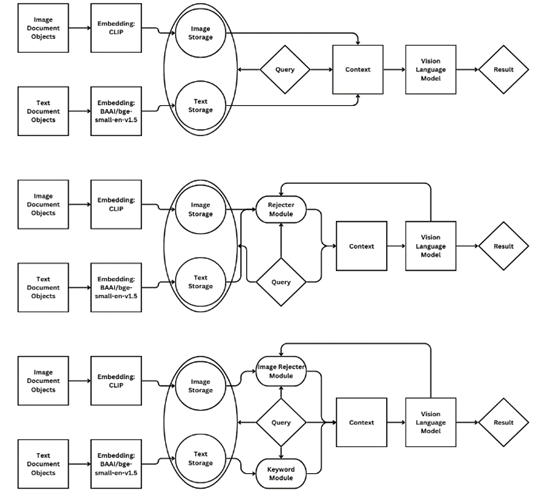
\includegraphics[width=1\linewidth]{image.png}
    \caption{Naive RAG pipeline}
    \label{fig:enter-label}
\end{figure}

\subsection{Rejecter Module}
Furthermore, the modularity of our pipeline, induced by leveraging the LlamaIndex framework [4] to encapsulate the stages of indexing, storing, and retrieval, facilitated the integration of our proposed modules, which aimed to refine retrieved context by reducing noise, focusing on more crucial information post-retrieval.
The first module that was implemented was deemed the “Rejecter Module”, which addresses noise in the retrieved contextual information by selectively discarding irrelevant sources. In this module, the vision-language model is supplied with the source, its modality, and the query. It is then asked if the source can be used to sufficiently answer the query: “Can the following <source-modality>, where "-" representes an underscore, be used to answer the query ‘<query>’ Answer 'yes' or 'no'. <source>”. Objects deemed suitable as a source to respond to the query are passed along to be used as contextual information. Otherwise, the sources that are considered irrelevant by the VLM are discarded, enhancing the quality of the augmented query.
After its implementation, it was observed that it effectively filtered out irrelevant images. However, the module displayed an aggressive tendency in rejecting even the most relevant text snippets, which limited any passed textual information in the provided context for the augmented query.

\subsection{Keyword Module}
Inspired by the need to mitigate the Rejecter Module’s shortcomings in sufficiently rejecting noisy textual sources while also passing relevant ones, another module was created to be used in tandem an image-only modification to the Rejecter Module, deemed the “Keyword Module”. We employ spaCy [5], an open-source natural language processing framework, to parse the query and each retrieved textual source for keywords. After identifying noun keywords, stop words are removed by using a corpus of stop words, which are words appearing frequently in text, but carry little semantic meaning, such as “the”, “a”, or “of”. Then, term frequency-inverse document frequency (TF-IDF) is employed to rank the importance of keywords, assigning higher weights to terms that are frequent within the query, but rare in the context of all documents, which would be the retrieved textual sources. The top N keywords would be extracted from each textual source, and they would only be passed onto the augmented query if the number of intersecting keywords with the query surpass a threshold M. By prioritizing textual sources based on their keywords from TF-IDF analysis, the Keyword Module identifies the most important textual sources that align with the content of the query.
By using these proposed modules and integrating them into our RAG pipeline, we aimed to reduce noise and emphasize the relevance of contextual information seen by the VLM.

\begin{figure}
    \centering
    
\includegraphics[width=1\linewidth]{image2.png}
    \caption{Results from the MultimodalQA benchmark on the 'TextQ' and 'ImageQ' subsets.}
    \label{fig:enter-label}
\end{figure}

\begin{figure}
    \centering
    
\includegraphics[width=1\linewidth]{image3.png}
    \caption{Results from the WebQA benchmark. YesNo, Number, Color, and Shape are image query categories.}
    \label{fig:enter-label}
\end{figure}

\section{Results}
\subsection{Implementation Details}
In our implementation, CLIP [6] was employed for image embeddings, while BAAI/bge-smal-en-v1.5 [7] was used as a text embedding model. For the vision-language model component, LLaVA-1.5 [8] was used. However, it is important to note that the modularity of our entire pipeline enables the seamless substitution of this model with any other multi-modal large language model capable of interpreting images and text simultaneously. This flexibility would allow for easy integration of state-of-the-art models or additional adapters/modules in the future.

\subsection{Dataset}
For evaluation, MultimodalQA and WebQA were used, which are question-answering datasets that require joint reasoning over text and images. They specifically can be summarized by the following formulation: Given a question \(Q\) and a list of sources \(s=\{s_1,s_2,\ldots\}\), the system would identify which sources should be used to answer the provided question and generate its associated answer. Although the MultimodalQA benchmark has questions with corresponding source lists containing table information, we only considered questions having types “TextQ” and “ImageQ”, which are denoted as “Text” and “Image” respectively in Table 1. Questions would require a single image or text source to answer sufficiently, whereas a couple image or text sources could be required in the WebQA benchmark, where questions requiring image sources have the following categories: “YesNo”, “number”, “color”, and “shape”. We evaluate the performance of retrieved and read sources, the sources used as contextual information provided to the VLM among the set of retrieved sources, via retrieval-F1 scores. As for the comparison between predicted and ground truth answers, keyword matching F1 scores were used based on the number of common keywords present in both answers. For consistency in each benchmark, 5 text sources and 3 image sources were retrieved for all model/pipeline configurations.


\subsection{Experiments}
We established baseline performance metrics using two scenarios. The first baseline involves using LLaVA-1.5 viewing only queries, without any access to external sources. This would provide insight into the inherent capabilities of the model operating without retrieval augmented generation. Then, the second baseline involved using a naïve RAG pipeline, where LLaVA-1.5 was coupled with a basic pipeline capable of indexing, storing, and retrieving document objects, but lacked any modules for noise reduction. This would help us gauge the performance impact of our proposed modules.

\begin{figure}
    \centering
    
\includegraphics[width=1\linewidth]{image4.png}
    \caption{Effects of Keyword Module parameters on MultimodalQA pipeline performance.}
    \label{fig:enter-label}
\end{figure}

\begin{figure}
    \centering
    
\includegraphics[width=1\linewidth]{image5.png}
    \caption{Effects of Keyword Module parameters on WebQA pipeline performance.}
    \label{fig:enter-label}
\end{figure}

Table 1 displays the results from the MultimodalQA benchmark on the ‘TextQ’ and ‘ImageQ’ subsets. It is evident that the inclusion of RAG generally improves performance. The addition of the Rejecter Module (RM) results in a significant improvement in image-source related queries, but the performance for text-source related queries drops, due to the module’s aggressive rejection of textual sources, resulting in a lower “Read” performance. In modifying the Rejecter Module to be image-only (IRM) and using the Keyword Module (KM) with the consideration of the top 100 keywords with a common keyword threshold of 3, these modules contribute to noticeable improvements across all categories, yielding a 57% increase in overall question-answering performance compared to the naïve RAG pipeline, showing the positive effects of reducing noise within contextual information provided to the VLM. With the Image-only Rejecter Module, in the case that it would reject every obtained image, the image with the highest similarity score with the query would be chosen as a backup.
In Table 2, we observe the performance of the pipeline configurations, where the KM considers the top 30 keywords with a common keyword threshold of 1, on the WebQA benchmark, which poses a more challenging task than MultimodalQA. Although the addition of the IRM and KM marginally improve overall question answering performance, it is not as significant as shown in the MultimodalQA benchmark, which is due to a couple of factors. WebQA presents queries that demand a deeper understanding of both textual and visual information, such as observing the shape or number of objects in an image, rather than with trivia-style questions, like in MultimodalQA. Also, compared to MultimodalQA, where the textual sources have an average word count of 88 words, the textual sources in WebQA are shorter, averaging 45 words. The stark difference in text lengths can impact the effectiveness of keyword extraction, which relies on the presence of sufficient textual content. Therefore, it is plausible that the observed minor increase in text performance in the WebQA benchmark could be attributed to the limitations induced by the shorter length of textual sources. 

\subsection{Ablation Study}
Table 3 displays different the effects of using different combinations in considering the top N keywords in retrieved textual sources with a variable common keyword threshold of M in the Keyword Module with the pipeline utilizing the Image-only Rejecter Module and the Keyword Module. As the threshold increases, more noise is reduced, where considering the top 100 keywords with a common keyword threshold of 3 increases overall question-answering performance the most on the MultimodalQA dataset.

Table 4 displays similar configurations on the WebQA dataset. However, we see that on this benchmark in particular that the best combination for text is (30,1), yet a higher ‘Read’ F1-scores are yielded with some configurations with a larger common keyword threshold. In these configurations, noise was reduced more, but more positive sources were discarded. Compared to the previous table, the lack of consistency in performance is likely due to the difficulty of the WebQA dataset and differences between the distributions of unique word counts of textual sources in both benchmarks

\begin{figure}
    \centering
    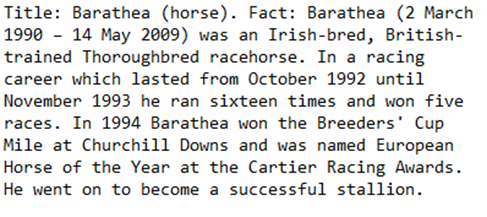
\includegraphics[width=1\linewidth]{image6.png}
    \caption{An example of a correctly accepted textual source by the Keyword Module from the MultimodalQA dataset, having the associated query “What award did Barathea win at Churchill Downs in 1994?” With the above source, LLaVA-1.5 responded correctly: “Barathea won the Breeders' Cup Mile at Churchill Downs in 1994."}
    \label{fig:enter-label}
\end{figure}

\begin{figure}
    \centering
    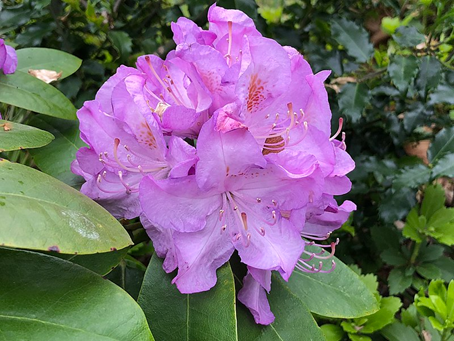
\includegraphics[width=1\linewidth]{image7.png}
    \caption{An example of a correctly accepted image source by the Image-only Rejecter Module from the WebQA dataset, having the associated query “Does a Minnetonka Rhododendron flower have petals in a cup shape?” With the above source, LLaVA-1.5 responded incorrectly, stating “Yes.”}
    \label{fig:enter-label}
\end{figure}

\begin{figure}
    \centering
    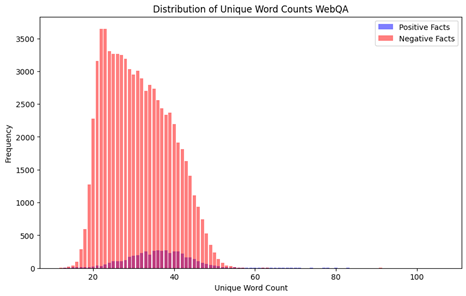
\includegraphics[width=1\linewidth]{image8.png}
    \caption{The distribution of unique word counts in textual sources in the WebQA dataset.}
    \label{fig:enter-label}
\end{figure}

\begin{figure}
    \centering
    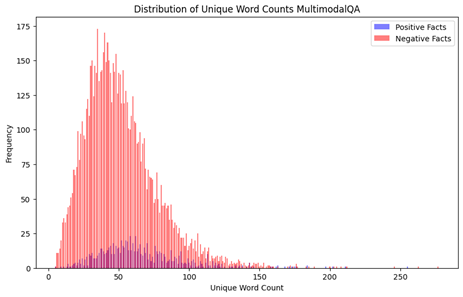
\includegraphics[width=1\linewidth]{image9.png}
    \caption{The distribution of unique word counts in textual sources in the WebQA dataset.}
    \label{fig:enter-label}
\end{figure}

\section{Conclusion}
In this work, we propose a modular retrieval-augmented generation pipeline capable of multimodal question-answering tasks, integrating novel modules to reduce noise and enhance contextual relevance post-retrieval. Our experiments on the MultimodalQA and WebQA benchmarks show the efficacy of our approach in improving question-answering performance across questions requiring textual or visual sources. The Rejecter Module, Image-only Rejecter Module, and Keyword Module played pivotal roles in reducing noise and emphasizing relevant information, resulting in performance improvements when compared to a naïve RAG pipeline without any additional modules. While our approach yielded promising results, challenges and limitations were encountered, which include the impact of dataset/benchmark characteristics and the effectiveness of keyword extraction. Moving forward, we advocate for further exploration of noise-reduction optimization strategies. For example, since the image and textual storages are separate, the Image-only Rejecter Module and Keyword Module operate in parallel and may perhaps utilize similarity scores from the query to each source as a weight when considering which sources to pass onto the augmented query. In conclusion, our work contributes to the advancement of multimodal retrieval-augmented pipelines by introducing modular adapters that can be appended to a naïve RAG model to emphasize relevant sources.

\section{References}
[1]	Alon Talmor, Ori Yoran, Amnon Catav, Dan Lahav, Yizhong Wang, Akari Asai, Gabriel Ilharco, Hannaneh Hajishirzi, and Jonathan Berant. (2021). MultiModalQA: Complex Question Answering over Text, Tables and Images.

[2]	Yingshan Chang, Mridu Narang, Hisami Suzuki, Guihong Cao, Jianfeng Gao, and Yonatan Bisk. (2022). WebQA: Multihop and Multimodal QA.

[3]	Wenhu Chen, Hexiang Hu, Xi Chen, Pat Verga, and William W. Cohen. (2022). MuRAG: Multimodal Retrieval-Augmented Generator for Open Question Answering over Images and Text.

[4]	Liu, J. (2022). LlamaIndex. https://doi.org/10.5281/zenodo.1234

[5]	Honnibal, M., and Montani, I. (2017). spaCy 2: Natural language understanding with Bloom embeddings, convolutional neural networks and incremental parsing.

[6]	Alec Radford, Jong Wook Kim, Chris Hallacy, Aditya Ramesh, Gabriel Goh, Sandhini Agarwal, Girish Sastry, Amanda Askell, Pamela Mishkin, Jack Clark, Gretchen Krueger, and Ilya Sutskever. (2021). Learning Transferable Visual Models From Natural Language Supervision.

[7]	Shitao Xiao, Zheng Liu, Peitian Zhang, and Niklas Muennighoff. (2023). C-Pack: Packaged Resources To Advance General Chinese Embedding.

[8]	Haotian Liu, Chunyuan Li, Yuheng Li, and Yong Jae Lee. (2023). Improved Baselines with Visual Instruction Tuning.

\end{document}
